\section{Introduction}

The aim of this excercise is to learn the basics of emission and absorption
spectroscopy. The repport will be split into three sections. First of all,
three light bulbs; a diode-based, a halogen and an energy saving bulb, will be
investigated and compared to the spectra of that of a blackbody. The
temperature of the various light sources will be determined and so will they be
compared to the solar spectrum. 

As the recorded solar spectrum also contains absorption lines\footnote{Theese
    are narrow regions of decreased intensity as a result of photons being
absorbed in their path from the source to the detector.} (often reffered to as
Fraunhofer lines), as a result of the gas in the photosphere, we will determine
the wavelengths and identify the corresponding molecules, which consequently
must be in the outer layer of the sun (see \cref{fig:frauenhofer} In addition, theemission spectra from
spectral lamps and a laser will be studied. 
Look at the line spectra from such lamps and compare with a data base to assign
the initial and final electronic stats for as many lines as possible. 

\begin{figure}[h!]
    \centering
    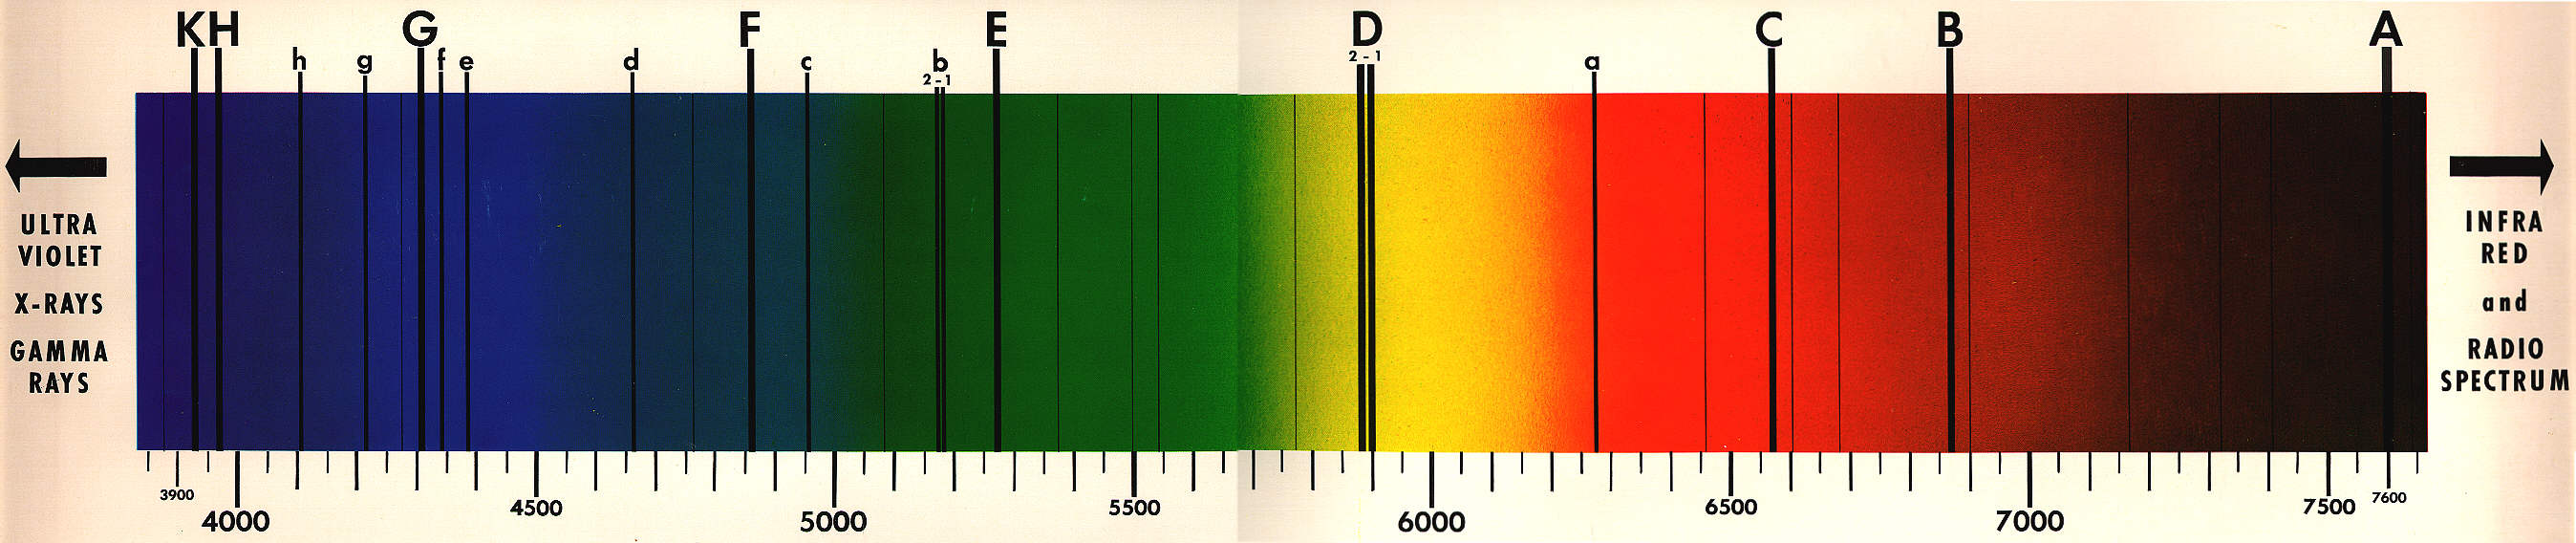
\includegraphics[width=0.5\textwidth]{solarspectrum}
    \caption{The solar spectrum}
    \label{fig:frauenhofer}
\end{figure}


